\section{ReLU's Over-approximation}

The Rectified Linear Unit (ReLU) activation function is a commonly used activation function in neural networks. It is defined as follows:

\vspace{5mm}
$ReLU(x) = max(0, x)$
\vspace{5mm}
\\
In other words, if the input to the ReLU function (x) is greater than zero, the output will be equal to the input. If the input is less than or equal to zero, the output will be zero.
\\
The ReLU function has a simple and computationally efficient implementation, which contributes to its popularity. It introduces non-linearity into the network, allowing neural networks to learn complex relationships between inputs and outputs. ReLU is particularly useful in deep neural networks as it helps alleviate the vanishing gradient problem, where gradients become very small during backpropagation, by allowing the gradient to flow more easily for positive inputs.

\begin{figure}[t]
	\caption{\label{fig:relu_types} Main used ReLU's convex approximation in the literaturet}
	\centering
	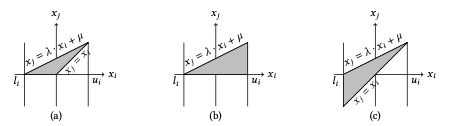
\includegraphics[scale=0.8]{"Chapter5/img/ReLU's/relus.png"}
\end{figure}


With regard to symbolic interval bound propagation the main problem that arises is that we often need to deal with networks formed by FC and ReLU. But we can't deal with it because it is not a linear and, therefore, we have to use a convex over-approximation. Below the main used convex over-approximation:

\begin{enumerate}
    \item The approximation of Fig. 4 (a) minimizes the area in the $x_i$ , $x_j$ plane, and would add the following relational constraints and concrete bounds for $x_j$:
       \begin{equation}
            \begin{aligned}
                & x_i \leq x_j, 0 \leq x_j, \\
                & x_j \leq u_i\left(x_i-l_i\right) /\left(u_i-l_i\right) . \\
                & l_j=0, u_j=u_i .
            \end{aligned}
        \end{equation}
        
 This ReLU approximation is the best possible in term of area but it has the disadvantage that uses 2 lower constraints. For this reason it is not well suitable for a further implementation in a bound propagation alghoritm.

    \item The approximation from Fig. 4 (b) adds the following constraints and bounds for $x_j$ :
    \begin{equation}
        \begin{aligned}
            & 0 \leq x_j \leq u_i\left(x_i-l_i\right) /\left(u_i-l_i\right), \\
            & l_j=0, u_j=u_i .
        \end{aligned}
    \end{equation}

    \item The approximation from Fig. 4 (c) adds the following constraints and bounds:
    \begin{equation}
        \begin{aligned}
            x_i & \leq x_j \leq u_i\left(x_i-l_i\right) /\left(u_i-l_i\right), \\
            l_j & =l_i, u_j=u_i .
        \end{aligned}
    \end{equation}
\end{enumerate}

\subsection{Application of ReLU approximation to bound propagation}
The networks used for verification purposes are typically small and typically consist of fully connected layers and ReLU activation layers. Earlier, we explained the process of bound propagation for networks composed solely of fully connected layers, referred to as Symbolic Interval propagation. Now, let's discuss how to modify the bound propagation method to make it compatible with ReLU layers.

Consider a network composed of three fully connected (FC) layers with dimensions 2x2, along with two ReLU layers, as shown in Figure 5 of the paper titled "Optimized Symbolic Interval Propagation for Neural Network Verification."


\begin{figure}[t]
	\caption{\label{fig:fc_relu_network} Simple neural network with FC and ReLU}
	\centering
	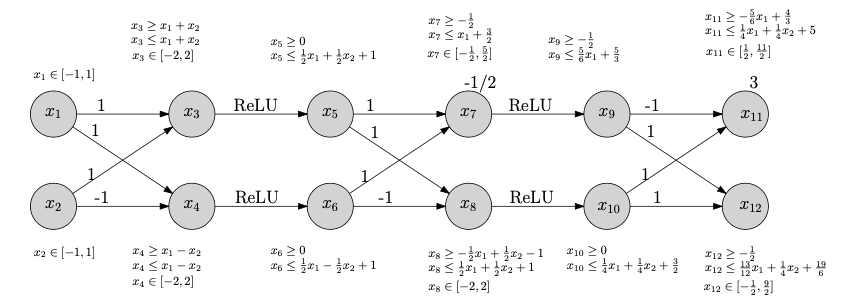
\includegraphics[scale=0.6]{"Chapter5/img/network_with_bound_prop/network_with_bound_prop.png"}
\end{figure}


To incorporate ReLU layers into the bound propagation process, we need to account for the behavior of the ReLU activation function. Below are the steps to modify bound propagation for networks containing ReLU layers:

\begin{enumerate}
	\item Symbolic Interval Propagation (SIP) with Fully Connected (FC) Layers:

	\begin{itemize}
		\item Initially, we start with an input layer, where the input bounds are represented symbolically.
		\item For each FC layer, we calculate the affine transformation symbolic bounds as seen previously.
		\item The numeric output bounds of the FC layer are obtained through the concretization operation of the symbolic bounds and input bounds
	\end{itemize}

	\item Incorporating ReLU layers:

		\begin{itemize}
			\item After each FC layer, introduce a ReLU layer, which applies the ReLU activation function element-wise to the output of the FC layer.
		\end{itemize}

	\item Bound Propagation through ReLU Layers

		\begin{itemize}
			\item For each ReLU layer, we compute the lower and upper bounds of the output based on the input bounds.
			\item If the lower bound of the input is greater than zero, the lower bound of the output remains the same as the lower bound of the input. This is intuitive because if the lower bound is greater that zero then we can ignore the ReLU 						second dial of the Carthesian plan and treat it as a simple bisector of the first quadrant.
			\item If the upper bound of the input is less than or equal to zero, the upper bound of the output is zero. This is intuitive because if the upper bound il less that zero than we can ignore the ReLU first dial of the Carthesian  plan and 						treat it as a simple zero function.
			\item If the lower bound is less than zero and the upper bound is greater than 0 then it is needed to apply an over-approximation of the ReLU symbolic bounds.\\
				In the example in the Fig ~\ref{fig:fc_relu_network} all the neurons are in the third case and it is used the following metric for the linearization:\\
				If $u<\lvert l \rvert$ is applied the ReLU over-approximation in Fig~\ref{fig:relu_types} b\\
				 Else If  $u>\lvert l \rvert$ is applied the ReLU over-approximationin in Fig~\ref{fig:relu_types} c\\
				This diversification in the over-approximation's choice is due to the fact that  if  $u<\lvert l \rvert$ the over-approximation in Fig~\ref{fig:relu_types} b introduces a smaller error than the one in  Fig~\ref{fig:relu_types} c and 						vice-versa. The over-approximation of the ReLU introduces a discrepancy between the symbolically propagated limits and the actual value limits, causing a potential over-estimation errors in limit propagation which increases as 						the number of ReLu layers increases and consequently as the depth of the network increases.
		\end{itemize}

	\item Iterative process:

		\begin{itemize}
			\item Apply the modified bound propagation process iteratively across all FC and ReLU layers in the network.
			\item The output bounds obtained from the last FC layer represent the output bounds of the network.
		\end{itemize}
\end{enumerate}

\subsection{Detailed Study of Symbolic Linear Relaxation of ReLU}
\label{subsec:symbolic-linear-relaxation}
The key insight of symbolic linear relaxation is to find the tightest linear bounds for the ReLU function, minimizing the overestimation error when approximating network outputs. However, it is important to note that the approximation errors may vary for overestimated nodes in different layers, depending on the symbolic intervals assigned as inputs.

For layers preceding the $n_0$-th layer, which is the first layer with overestimated nodes, all nodes have the same symbolic lower and upper bounds as you can notice in the first ReLU layer of the example.

However, in deeper layers where overestimated nodes become more frequent, the expressions for the lower and upper symbolic bounds can be more complex. To address this challenge, we provide a detailed discussion and illustration of how symbolic linear relaxation works.
The linearization below in not present in section 2, but it is the tightest linearization possible and it is the one that will be used in the bound propagation. This is due to the fact that it introduces the smallest error possible respect to the linearizations seen before.

Let's consider an arbitrary overestimated node A, with the equation given by $z = Relu(Eq)$, where $Eq$ represents its input kept as a symbolic interval $[Eq_{low}, Eq_{up}]$. Additionally, let $n_0$ represent the first layer where overestimated nodes occur, $n_A$ denote the layer in which node A appears, and $(l_{low}, u_{low})$ and $(l_{up}, u_{up})$ represent the concrete lower and upper bounds of A's symbolic bounds $Eq_{low}$ and $Eq_{up}$.

We can consider several cases for the symbolic linear relaxations applied to node A, depending on its position relative to the $n_0$ layer.
    
\begin{enumerate}
        \item if $n_0 == n_A$: if A is an overstimed node in $n_0$ than we see that A's input equation $Eq$ satisfies $Eq_{low} = Eq_{up}=Eq$ .  Due to the fact that $u>0$ and $l<0$ the output can be approximated with:
        \begin{equation}
       	 \operatorname{Relu}([E q, E q]) \mapsto\left[\frac{u}{u-l} E q, \frac{u}{u-l}(E q-l)\right]
        \end{equation}
        
        \item $n_A>n_0$ : If $\mathrm{A}$ is an overestimated node after $n_0$-th layer, 
    	possibly its symbolic lower bound equation $E q_{l o w}$ is no longer the same as its upper bound equation $E q_{u p}$ before relaxation.
     	Though we can still approximate the it as $\operatorname{Relu}\left(\left[E q_{l o w}, E q_{u p}\right]\right) \mapsto\left[\frac{u_{u p}}{u_{u p}-l_{l o w}} E q_{l o w}, \frac{u_{u p}}{u_{u p}-l_{l o w}}\left(E q_{u p}-l_{\text {low }}\right)\right]$, this is not 		 	the tightest 	possible bound. Therefore, we consider bounds on $E q_{l o w}$ and $E q_{u p}$ independently to achieve tighter approximations.
	\begin{equation}
    		\begin{aligned}
    			& \operatorname{Relu}\left(\left[E q_{\text {low }}, E q_{u p}\right]\right) \mapsto \\
    			& \qquad\left\{\begin{array}{l}
    				{\left[0, \frac{u_{u p}}{u_{u p}-l_{u p}}\left(E q_{u p}-l_{u p}\right)\right] \quad\left(l_{\text {low }} \leq 0, l_{u p} \leq 0, u_{l o w} \leq 0, u_{u p}>0\right)} \\
    				{\left[0, E q_{u p}\right] \quad\left(l_{\text {low }} \leq 0, l_{u p} \leq 0, u_{l o w}>0, u_{u p}>0\right)} \\
    				{\left[\frac{u_{l o w}}{u_{l o w}-l_{l o w}} E q_{l o w}, \frac{u_{u p}}{u_{u p}-l_{u p}}\left(E q_{u p}-l_{u p}\right)\right] \quad\left(l_{\text {low }} \leq 0, l_{u p}>0, u_{l o w} \leq 0, u_{u p}>0\right)} \\
    				{\left[\frac{u_{\text {low }}}{u_{\text {low }}-l_{l o w}} E q_{l o w}, E q_{u p}\right] \quad\left(l_{\text {low }} \leq 0, l_{u p} \leq 0, u_{l o w}>0, u_{u p}>0\right)}
   			\end{array}\right.
   		\end{aligned}
%    	
	\end{equation}
 \end{enumerate}
    